% !TeX spellcheck = cs_CZ
%{\tikzset{external/prefix={tikz/FYZII/}}
% \tikzset{external/figure name/.add={ch35_}{}}
%---------------------------------------------------------------------------------------------------
% file fey2ch35.tex
%---------------------------------------------------------------------------------------------------
%=========================== Kapitola Paramagnetizmus a magnetická rezonance =======================
\setchaptertoc
\chapter{Paramagnetizmus a magnetická rezonance}\label{fyz:IIchapXXXV}

  \section{Kvantové magnetické stavy}\label{fyz:IIchapXXXVsecI}
  \section{Sternův-Gerlachův pokus}\label{fyz:IIchapXXXVsecII}
  \section{Rabiho metoda molekulového svazku}\label{fyz:IIchapXXXVsecIII}
  \section{Paramagnetizmus makroskopických látek}\label{fyz:IIchapXXXVsecIV}
  \section{Chlazení pomocí adiabatické demagnetizace}\label{fyz:IIchapXXXVsecV}
  \section{Jaderná magnetická rezonance}\label{fyz:IIchapXXXVsecVI}
  \section{Příklady a cvičení}\label{fyz:IIchapXXXVsecVII}

    \begin{figure}[ht!] %\ref{fyz:fig846}
      \centering
      \subcaptionbox{\label{fyz:fig846a}}{\luafigure[0.9]{fyz_fig846a.pdf}}               \newline
      \subcaptionbox{\label{fyz:fig846b}}{\luafigure[0.9]{fyz_fig846b.pdf}}               \newline
      \subcaptionbox{\label{fyz:fig846c}}{\luafigure[0.9]{fyz_fig846c.pdf}}
      \caption{
               (\cite[s.~748]{Feynman02})}
      \label{fyz:fig846}
    \end{figure}

    \begin{figure}[ht!] %\ref{fyz:fig847}
      \centering
      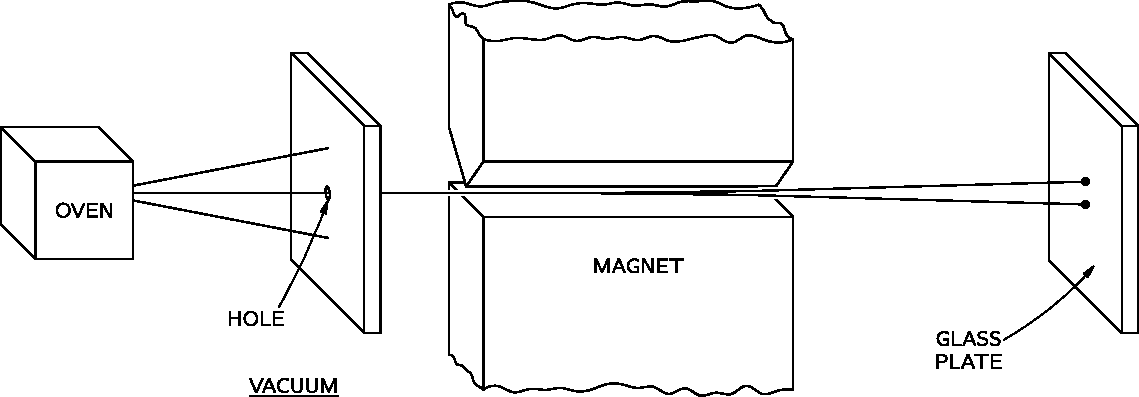
\includegraphics[width=0.7\linewidth]{fyz_fig847.pdf}
      \caption{
               (\cite[s.~707]{Feynman02})}
      \label{fyz:fig847}
    \end{figure}

    \begin{figure}[ht!] %\ref{fyz:fig848}
      \centering
      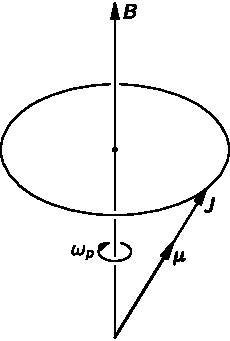
\includegraphics[width=0.7\linewidth]{fyz_fig848.pdf}
      \caption{
               (\cite[s.~707]{Feynman02})}
      \label{fyz:fig848}
    \end{figure}

    \begin{figure}[ht!] %\ref{fyz:fig849}
      \centering
      \subcaptionbox{\label{fyz:fig849a}}{\luafigure[0.9]{fyz_fig849a.pdf}}               \newline
      \subcaptionbox{\label{fyz:fig849b}}{\luafigure[0.9]{fyz_fig849b.pdf}}
      \caption{
               (\cite[s.~748]{Feynman02})}
      \label{fyz:fig849}
    \end{figure}

    \begin{figure}[ht!] %\ref{fyz:fig850}
      \centering
      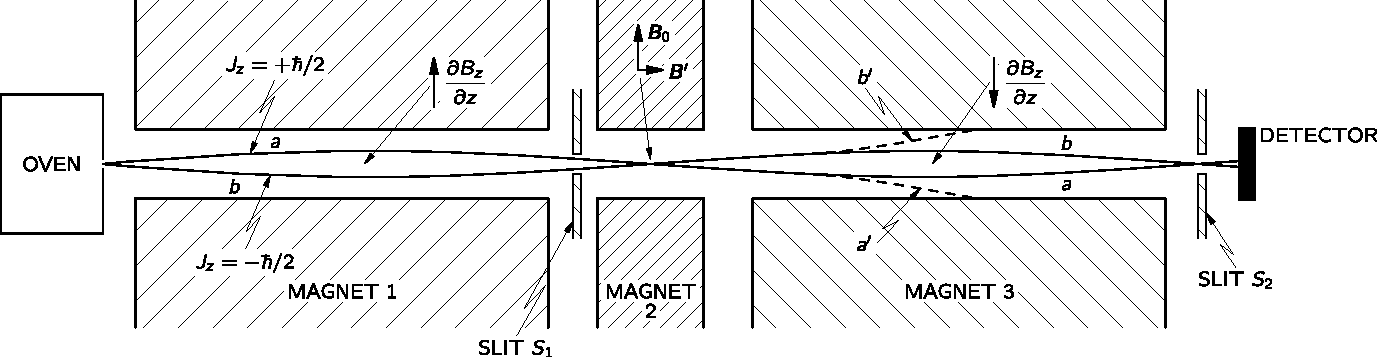
\includegraphics[width=0.7\linewidth]{fyz_fig850.pdf}
      \caption{
               (\cite[s.~707]{Feynman02})}
      \label{fyz:fig850}
    \end{figure}

    \begin{figure}[ht!] %\ref{fyz:fig851}
      \centering
      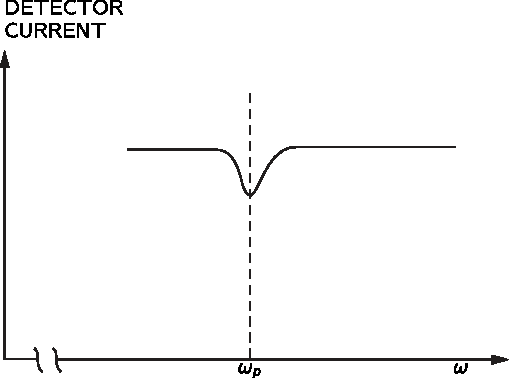
\includegraphics[width=0.7\linewidth]{fyz_fig851.pdf}
      \caption{
               (\cite[s.~707]{Feynman02})}
      \label{fyz:fig851}
    \end{figure}

    \begin{figure}[ht!] %\ref{fyz:fig852}
      \centering
      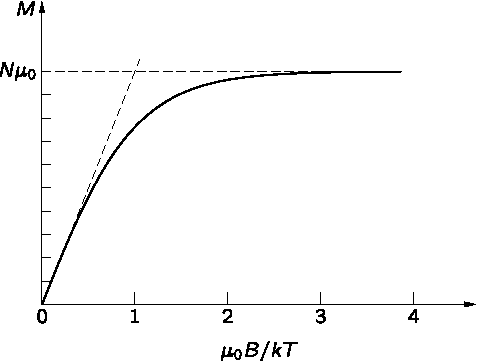
\includegraphics[width=0.7\linewidth]{fyz_fig852.pdf}
      \caption{
               (\cite[s.~707]{Feynman02})}
      \label{fyz:fig852}
    \end{figure}

    \begin{figure}[ht!] %\ref{fyz:fig853}
      \centering
      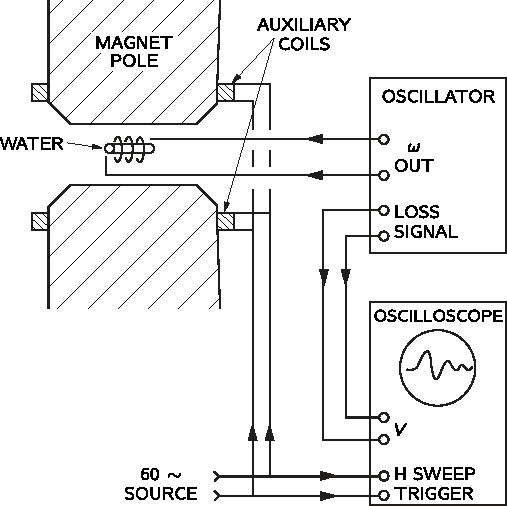
\includegraphics[width=0.7\linewidth]{fyz_fig853.pdf}
      \caption{
               (\cite[s.~707]{Feynman02})}
      \label{fyz:fig853}
    \end{figure}

    \todo[inline]{Kapitola fey2ch35 je nedodělaná, obsahuje pouze obrázky}
    
%} %tikzset
%---------------------------------------------------------------------------------------------------
